\documentclass[12pt]{article}

\usepackage{pablo}
\usepackage[a5paper,margin=2cm]{geometry}
\usepackage{enumerate}

\pagestyle{empty}
\begin{document}

  \section*{Généralités sur les fonctions --- DS}

  \begin{exercice}[Calcul d'images et d'antécédents --- 4 points]
    Soit $f$ la fonction définie par $f:x\mapsto \frac{1}{3x-1}$.
    \begin{enumerate}[(a)]
      \item Calculer $g(0)$.
      \item Quelle est l'image de $-1$ par $g$ ?
      \item Résoudre $g(x)=\frac{1}{5}$.
      \item Quels sont les antécédents de 0 par $g$ ?
    \end{enumerate}
  \end{exercice}

  \begin{exercice}[Lecture graphique --- 7 points] Voici la courbe
    représentative d'une fonction $g$ définie sur $\left[-0,5;4\right]$.
    \begin{center}
      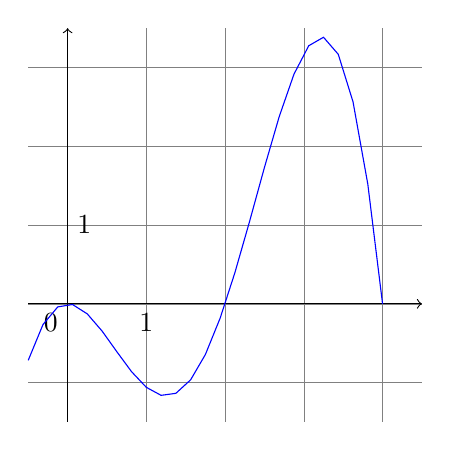
\begin{tikzpicture}[domain=-0.5:4.5, scale=1]
        \draw[very thin,color=gray,step=1] (-0.5,-1.5) grid (4.5,3.5);
        \draw[->] (-0.5,0) -- (4.5,0);
        \draw (1,0) node[below] {1};
        \draw[->] (0,-1.5) -- (0,3.5);
        \draw (0,1) node[right] {1};
        \draw (0,0) node[below left] {0};
        \draw[color=blue,domain=-0.5:4]
        plot (\x,{-6*(\x/2)*((\x/2)-1)*cos(45*\x + 90)});
      \end{tikzpicture}
    \end{center}

    \begin{enumerate}[{Question} 1 :]
      \item
        \begin{enumerate}[(a)]
          \item Dresser le tableau de variation de $g$.
          \item Quel est le minimum de $g$ sur son domaine de définition ?
          \item Quel est le maximum de $g$ sur $\left[-0,5;1\right]$ ?
        \end{enumerate}

      \item
        \begin{enumerate}[(a)]
          \item Combien vaut $g(1)$ ?
          \item Résoudre $g(x)=3$.
          \item Résoudre l'inéquation $g>1$ ?
        \end{enumerate}
    \end{enumerate}

  \end{exercice}

  \begin{exercice}[Représentation graphique --- 3 points]
    Tracer la courbe représentative de la fonction $h:x\mapsto
    \frac{x^2+3}{2x+1}$ sur $\left[0; 5\right]$ (faire apparaître les calculs
    ou un tableau de valeurs).

    %\begin{center}
    %  \begin{tikzpicture}[domain=-0.5:5.5, scale=1]
    %    \draw[very thin,color=gray,step=1] (-0.5,-0.5) grid (5.5,5.5);
    %    \draw[->] (-0.5,0) -- (5.5,0);
    %    \draw (1,0) node[below] {1};
    %    \draw[->] (0,-0.5) -- (0,5.5);
    %    \draw (0,1) node[right] {1};
    %    \draw (0,0) node[below left] {0};
    %    \draw[color=blue,domain=0:5] plot (\x,{(\x*\x+3)/(2*\x+1)});
    %  \end{tikzpicture}
    %\end{center}

  \end{exercice}

  \begin{exercice}[Problème --- 6 points]
    Lorsqu'un danger surgit sur la route, un laps de temps s'écoule entre la
    perception du danger par le conducteur et l'action musculaire de
    freiner. Il est appelé le temps de réaction. Sa durée est estimée à 1
    seconde.

    Pendant le temps de réaction, le véhicule continue à la même vitesse et
    parcourt une distance appelée distance de réaction.  La distance totale
    nécessaire au véhicule pour s'arrêter s'appelle la distance d'arrêt du
    véhicule. Elle s'obtient en ajoutant, à la distance de réaction, la
    distance de freinage, c'est-à-dire la distance parcourue entre le moment
    où commence le freinage et le moment où le véhicule s'arrête.  Pour la
    suite de l'exercice, on appellera $d$ la fonction qui lie la vitesse en km/h
    à la distance de freinage, en mètre.

    Sur route sèche, des études ont prouvé que la fonction d est définie par
    $d:v\mapsto \frac{v^2}{205}$.

    \begin{enumerate}[(a)]
      \item Donner les distances d’arrêt pour les vitesses (en km/h) suivantes~: 30 ; 50 ; 90 ; 110 ; 130.
      \item Un automobiliste roule en ville. Un ballon rebondit à 15 m de son véhicule. Il s’arrête en urgence.  Quelle vitesse ne devait-il pas dépasser pour éviter la collision ?
    \end{enumerate}

    \noindent Par temps de pluie, la fonction $d$ est définie par $d:v\mapsto
    \frac{v^2}{102}$. Répondre aux mêmes questions dans ce nouveau cas :

    \begin{enumerate}[(a)]
        \setcounter{enumi}{2}
      \item Donner les distances d’arrêt pour les vitesses (en km/h) suivantes~: 30 ; 50 ; 90 ; 110 ; 130.
      \item Un automobiliste roule en ville. Un ballon rebondit à 15 m de son véhicule. Il s’arrête en urgence.  Quelle vitesse ne devait-il pas dépasser pour éviter la collision ?
    \end{enumerate}

  \end{exercice}

  \begin{exercice}[Bonus] Trouver toutes les fonctions affines $f$ telles que
    $f\left(f\left(x\right)\right)=4x+3$ (rappel : une fonction affine est de
    la forme $f(x) = ax+b$).
  \end{exercice}

\end{document}
